Схема симулинк с добавлением ШИМ на  рис.\ref{fig:sim_final_VSS_PWM}. 
\begin{sidewaysfigure}[!h]\centering
	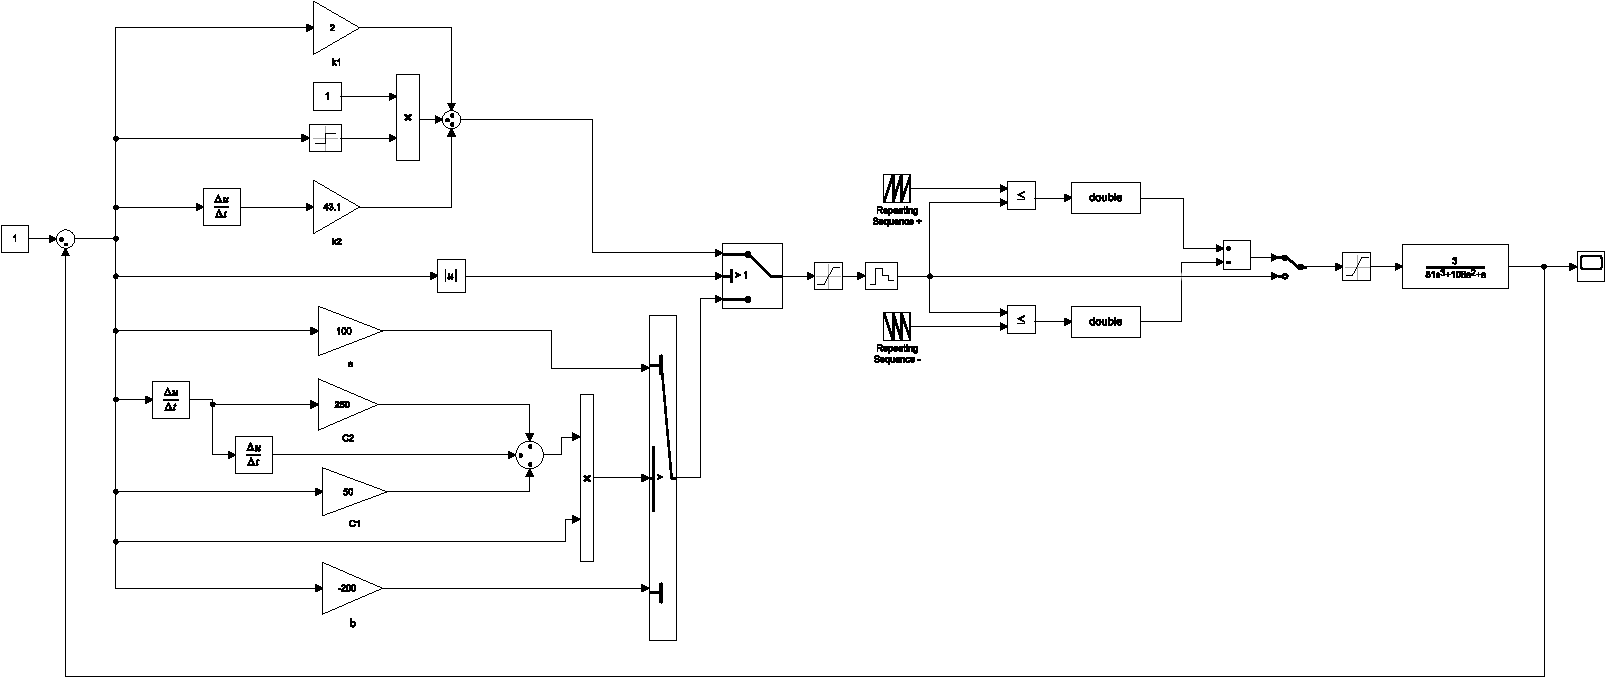
\includegraphics[width=1.0\linewidth]{images/sim_final_VSS_PWM}
	\caption{Структурная схема нелинейной СПС с ШИМ. }\label{fig:sim_final_VSS_PWM}
\end{sidewaysfigure}

%Рассмотрим влияние параметров схемы на ПП системы.
%Начнем с коэффициентов $K_1,K_2$, они работают при отклонении системы "в большом".
%Переходные процессы для разных значений этих параметров на рис.\ref{fig:final_VSS_PWM_k2},графики на всем интервале времени практически не изменяются, только в конце ПП при переключении систем управления появляются различия. Для более детального рассмотрения поакзана приближенная картинка на рис. \ref{fig:final_VSS_PWM_k2_zoom}.
%Они представлят собой коэффициенты пропорционального и дифференциального регулятора соответственно.
%Соответственно влияют они на систему также, как и коэффициенты ПД-регулятора в пункте \ref{title:PDR}: $k_1$ --- коэффициент пропорционального звена, влияет на скорость нарастания выходной величины, а $k_2$ --- коэффициент дифференцирующего звена, влияет на колебательность системы.
%При этом при разных сочетаниях коэффициентов время ПП практически не улучшается и наилучшее время составляет $133.46$ сек.
%\begin{figure}[!h]\centering
%	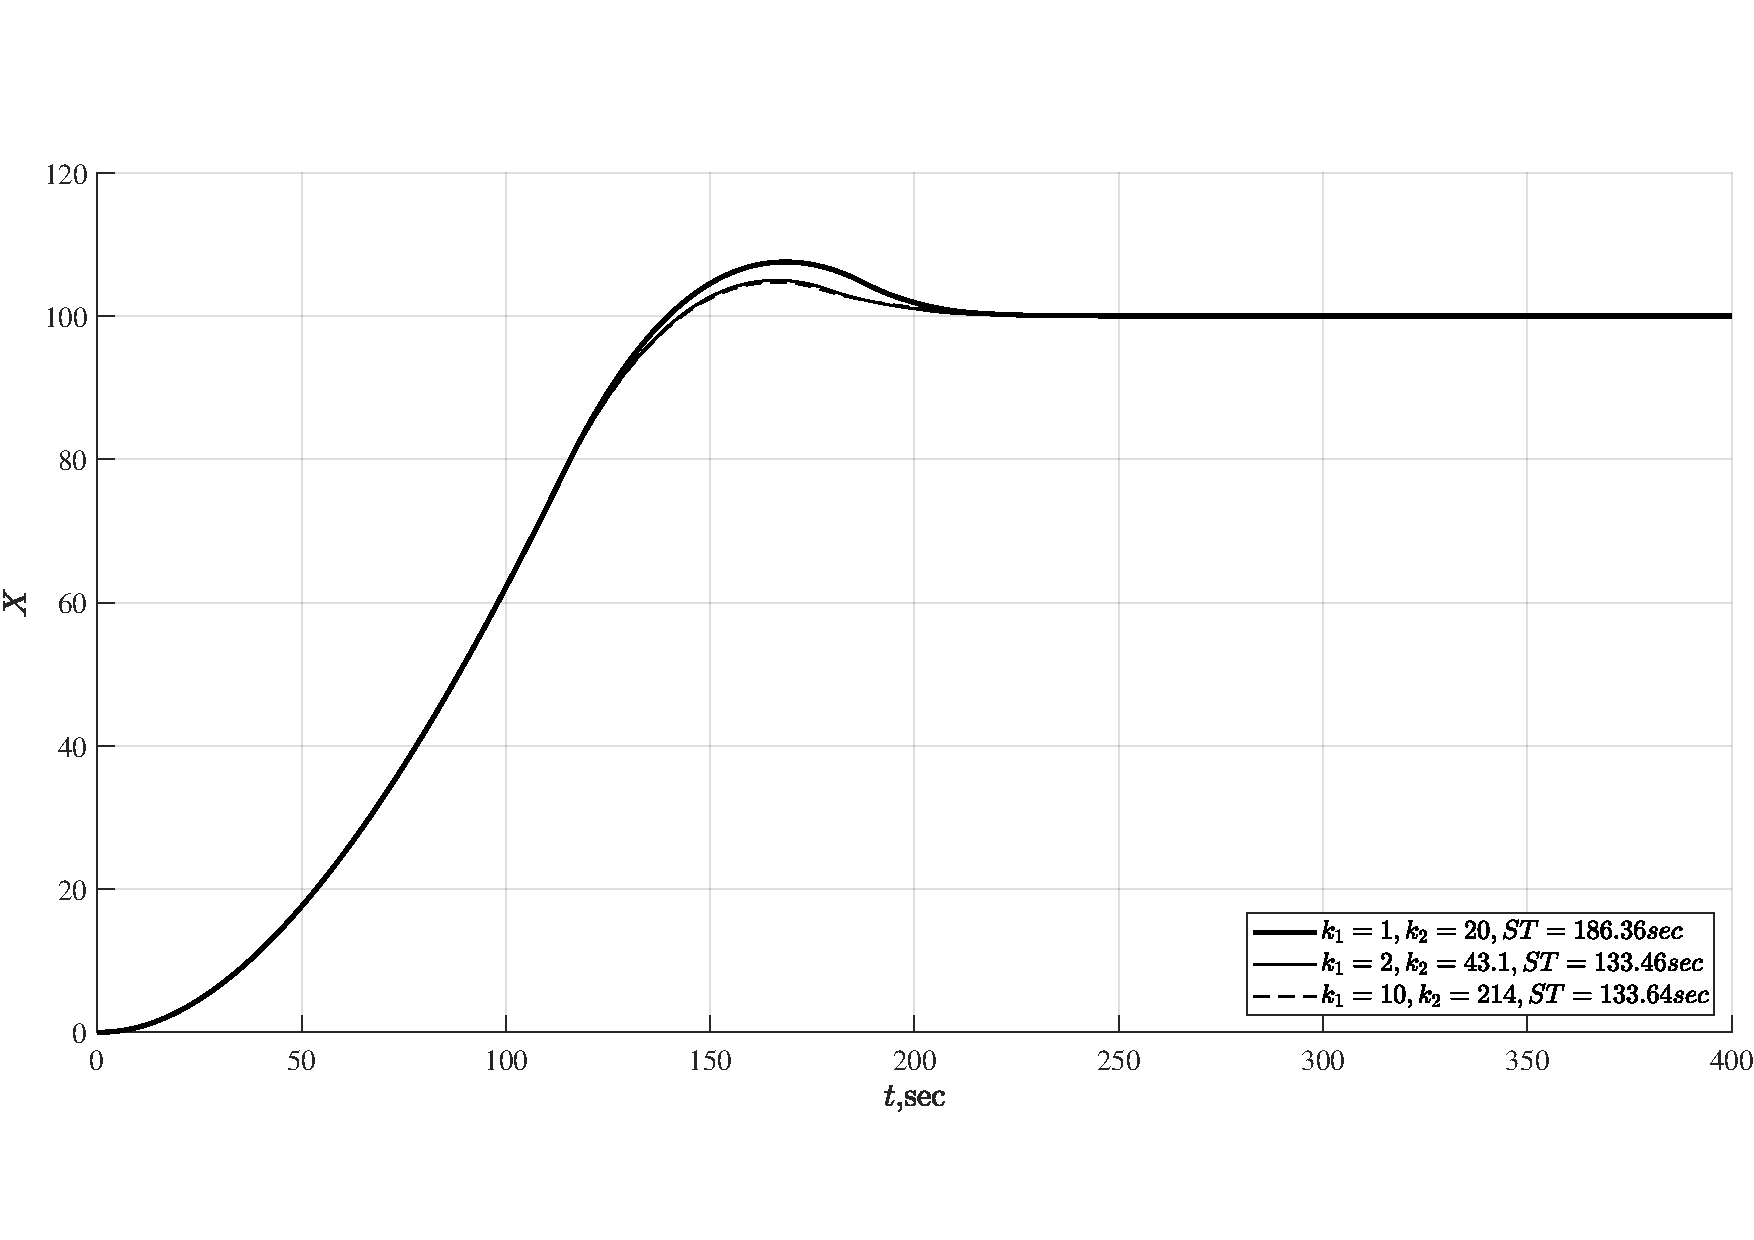
\includegraphics[width=1\linewidth]{images/final_VSS_PWM_k2}
%	\caption{ Графики ПП при вариации параметров $k_1,k_2$ в <<большом>>.}\label{fig:final_VSS_PWM_k2}
%\end{figure}
%\begin{figure}[!h]\centering
%	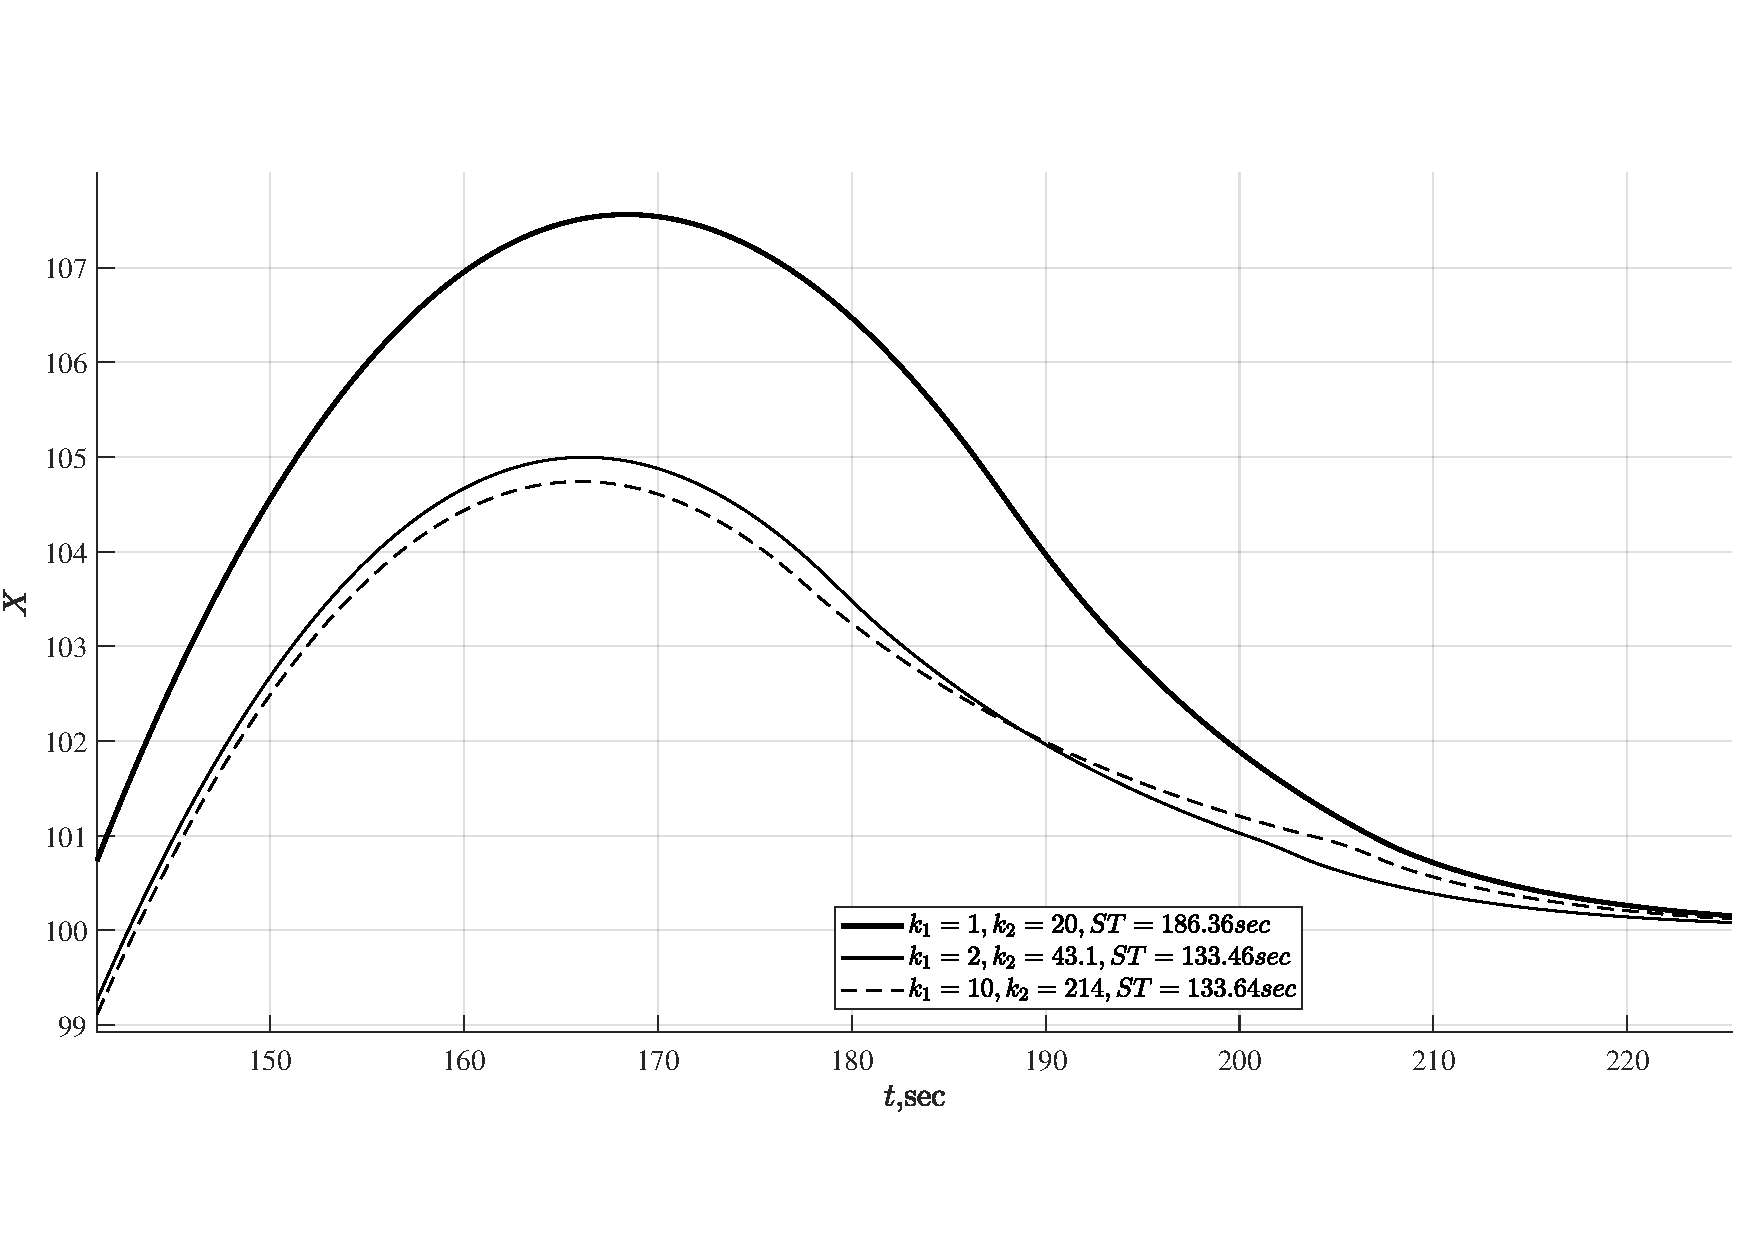
\includegraphics[width=1\linewidth]{images/final_VSS_PWM_k2_zoom}
%	\caption{ Приближенный график ПП при вариации параметров $k_1,k_2$.}\label{fig:final_VSS_PWM_k2_zoom}
%\end{figure}
%
%Теперь рассмотрим коэффициенты, влияющие на ПП "в малом": $C1,C2,a,b$. Также стоит отметить порог, отвечающий за переключение систем управления (переключение структур) при превышении абсолютными значениями ошибки данного порога. Данный порог определяет в какой момент переключить сруткуру, дргуими словами, он определяет при какие отклонения можно считать "большими", а какие "малыми". Так как при настройке системы отклонение "в малом" устанавливалось равным $1$, то и знаечние порога равно $1$. 
%Параметры $a$ и $b$ незначительно влияют на ПП ситемы при их отклонениях при правильной настройке.
%Это можно увидеть на рисунке \ref{fig:final_VSS_PWM_ab}.
%\begin{figure}[!h]\centering
%	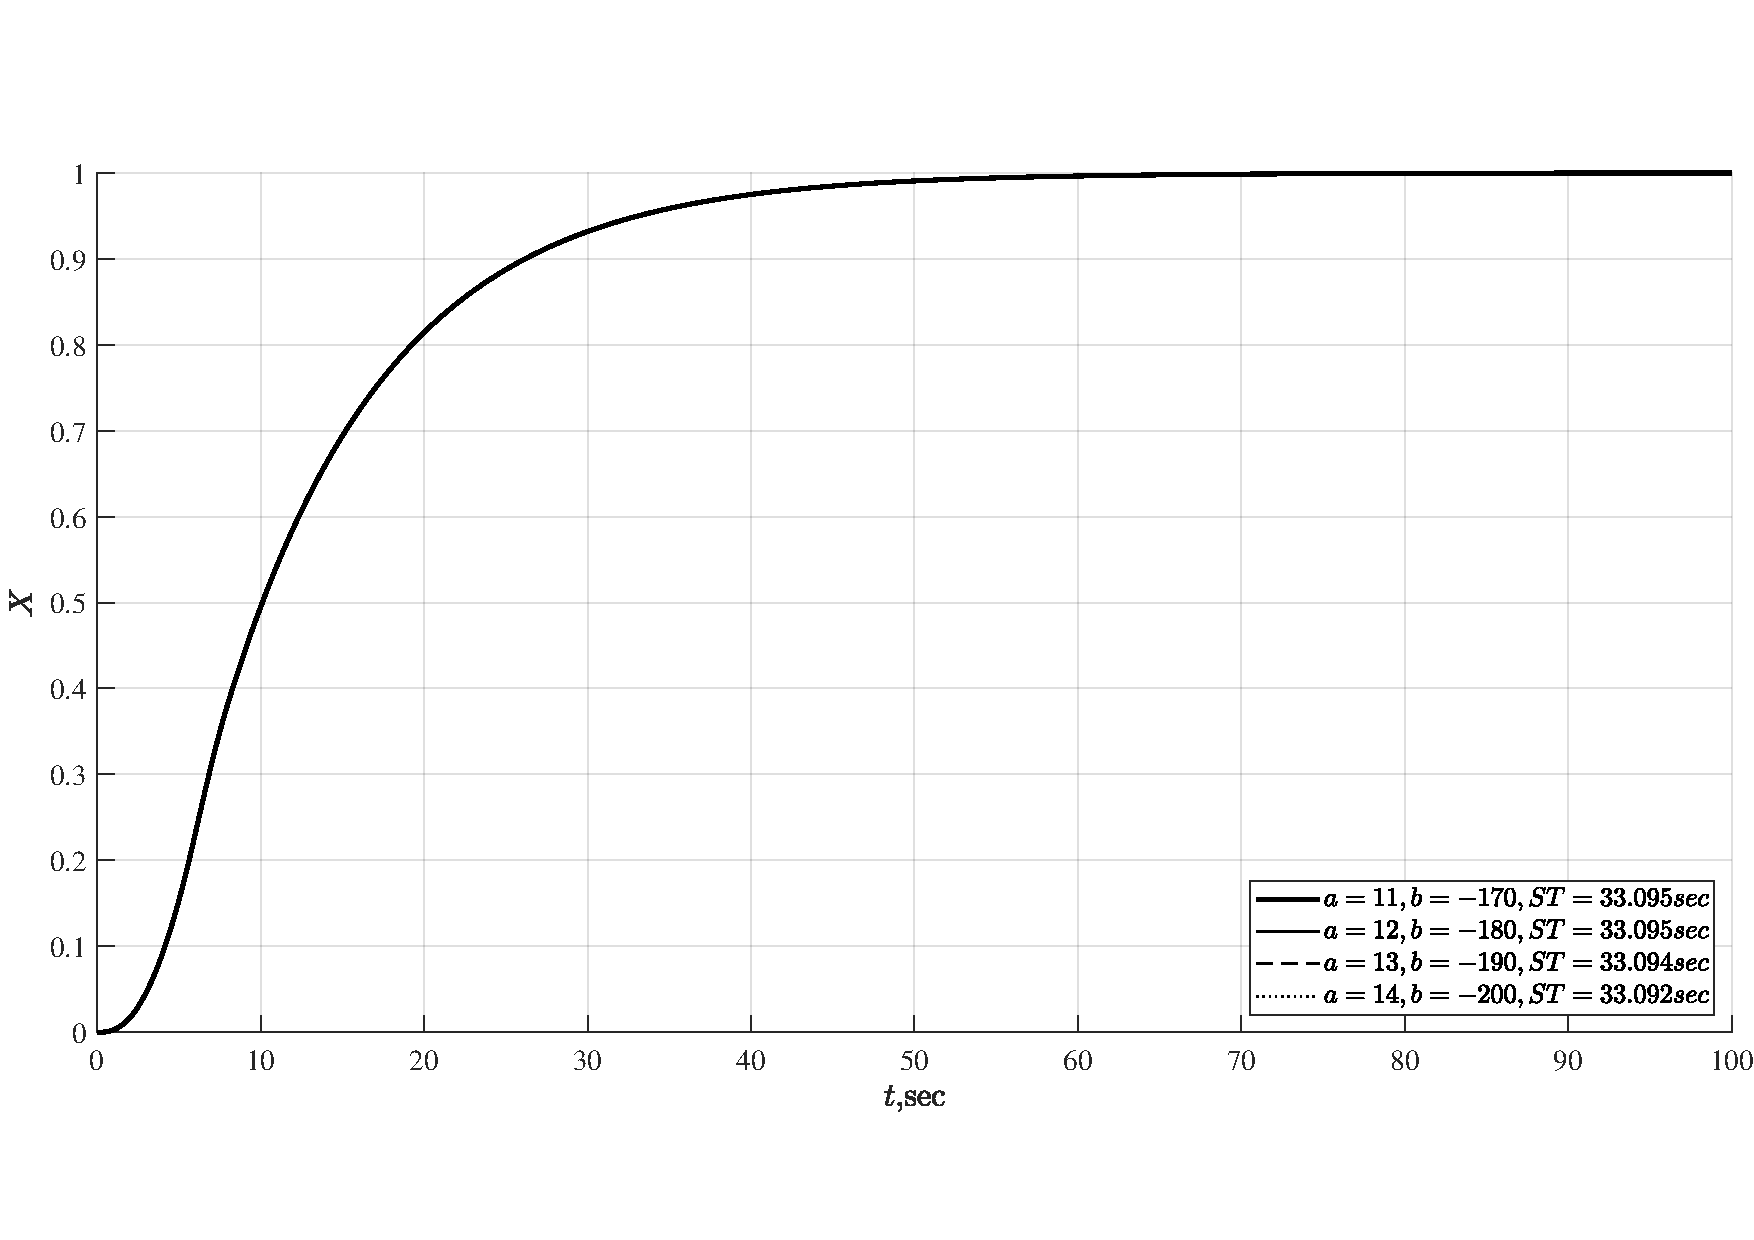
\includegraphics[width=1\linewidth]{images/final_VSS_PWM_ab}
%	\caption{ Графики ПП при вариации параметров $a,b$ в <<малом>>.}\label{fig:final_VSS_PWM_ab}
%\end{figure}
%Параметры $C1$ и $C2$ на колебательность и скорость нарастания. При увеличении $C1$ колебательность и скорость нарастания возрастает, а при увеличении $C2$ колебательность уменьшается. На рис. \ref{fig:final_VSS_PWM_c1c2} ПП ,  соответствующий техническим требованиям, при разных комбинациях параметров (На рис.\ref{fig:final_VSS_PWM_c1c2_zoom} в увеличенном масштабе). 
%\begin{figure}[!h]\centering
%	\includegraphics[width=1\linewidth]{images/final_VSS_PWM_c1}
%	\caption{ Графики ПП при вариации параметров $C1,C2$ в <<малом>>.}\label{fig:final_VSS_PWM_c1c2}
%\end{figure}
%\begin{figure}[!h]\centering
%	\includegraphics[width=1\linewidth]{images/final_VSS_PWM_c1_zoom}
%	\caption{ Графики ПП при вариации параметров $C1,C2$ в <<малом>>.}\label{fig:final_VSS_PWM_c1c2_zoom}
%\end{figure}
%
%При переходе к системе с ШИМ появляется постоянная ошибка и отрицательный выброс в противоположом с перерегулированием направлении
%, теперь коэффициент $a$ начинает играть решающее значение в виде ПП. Чем он ниже, тем больше отрицательный выброс. Также при увеличении коэфф. $a$ установившейся сигнал поднимается вше, тем самым уменьшается ошибка регулирования. На рис.\ref{fig:final_VSS_PWM_a} графики ПП при вариации параметров $a$ в <<малом>> в схеме с ШИМ(На рис.\ref{fig:final_VSS_PWM_a_zoom} в увеличенном масштабе).
При переходе к системе с ШИМ появляется постоянная ошибка
, теперь коэффициент $a$ начинает играть решающее значение в виде ПП. При увеличении коэфф. $a$ установившейся сигнал поднимается вше, тем самым уменьшается ошибка регулирования. На рис.\ref{fig:final_VSS_PWM_a} графики ПП при вариации параметров $a$ в <<малом>> в схеме с ШИМ(На рис.\ref{fig:final_VSS_PWM_a_zoom} в увеличенном масштабе).
\begin{figure}[!h]\centering
	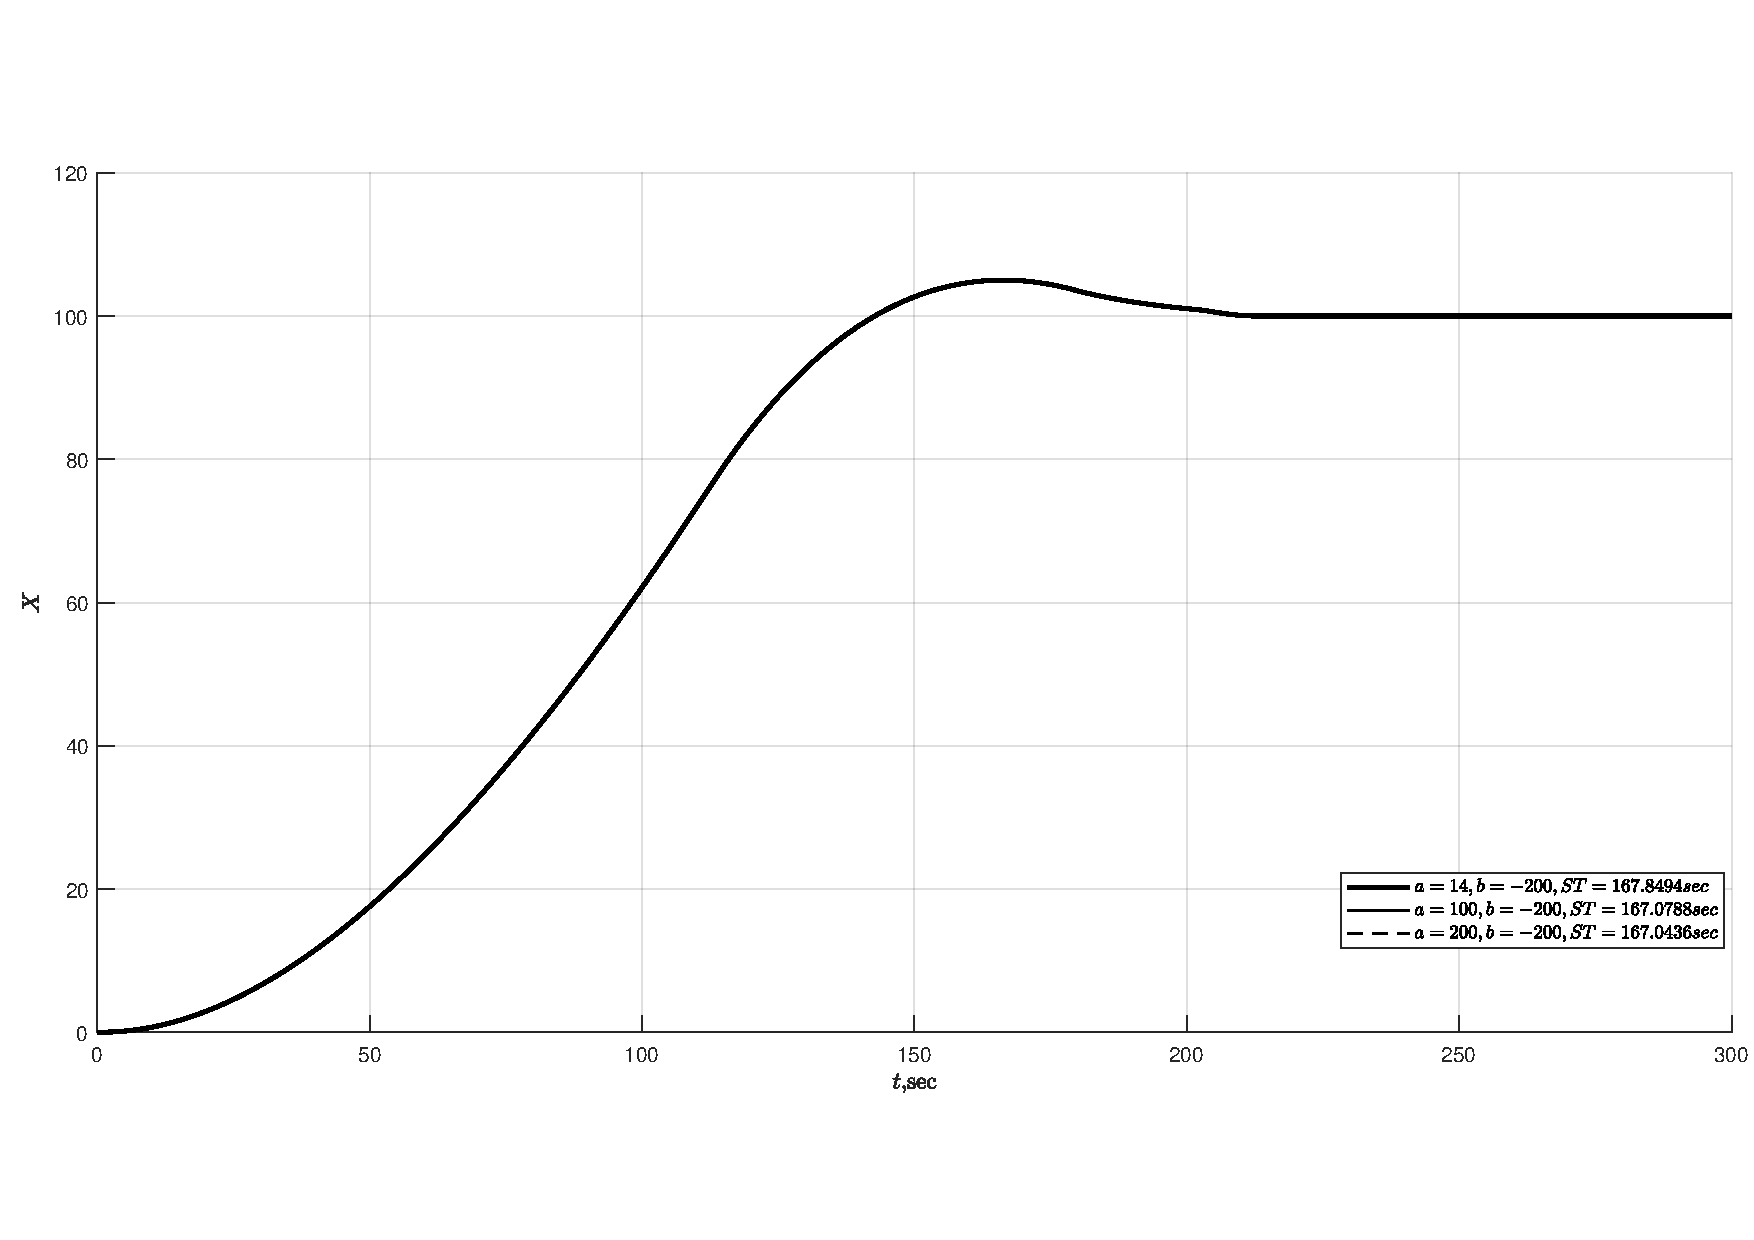
\includegraphics[width=1\linewidth]{images/final_VSS_PWM_a}
	\caption{ Графики ПП при вариации параметров $a$ в <<малом>> в схеме с ШИМ.}\label{fig:final_VSS_PWM_a}
\end{figure}
\begin{figure}[!h]\centering
	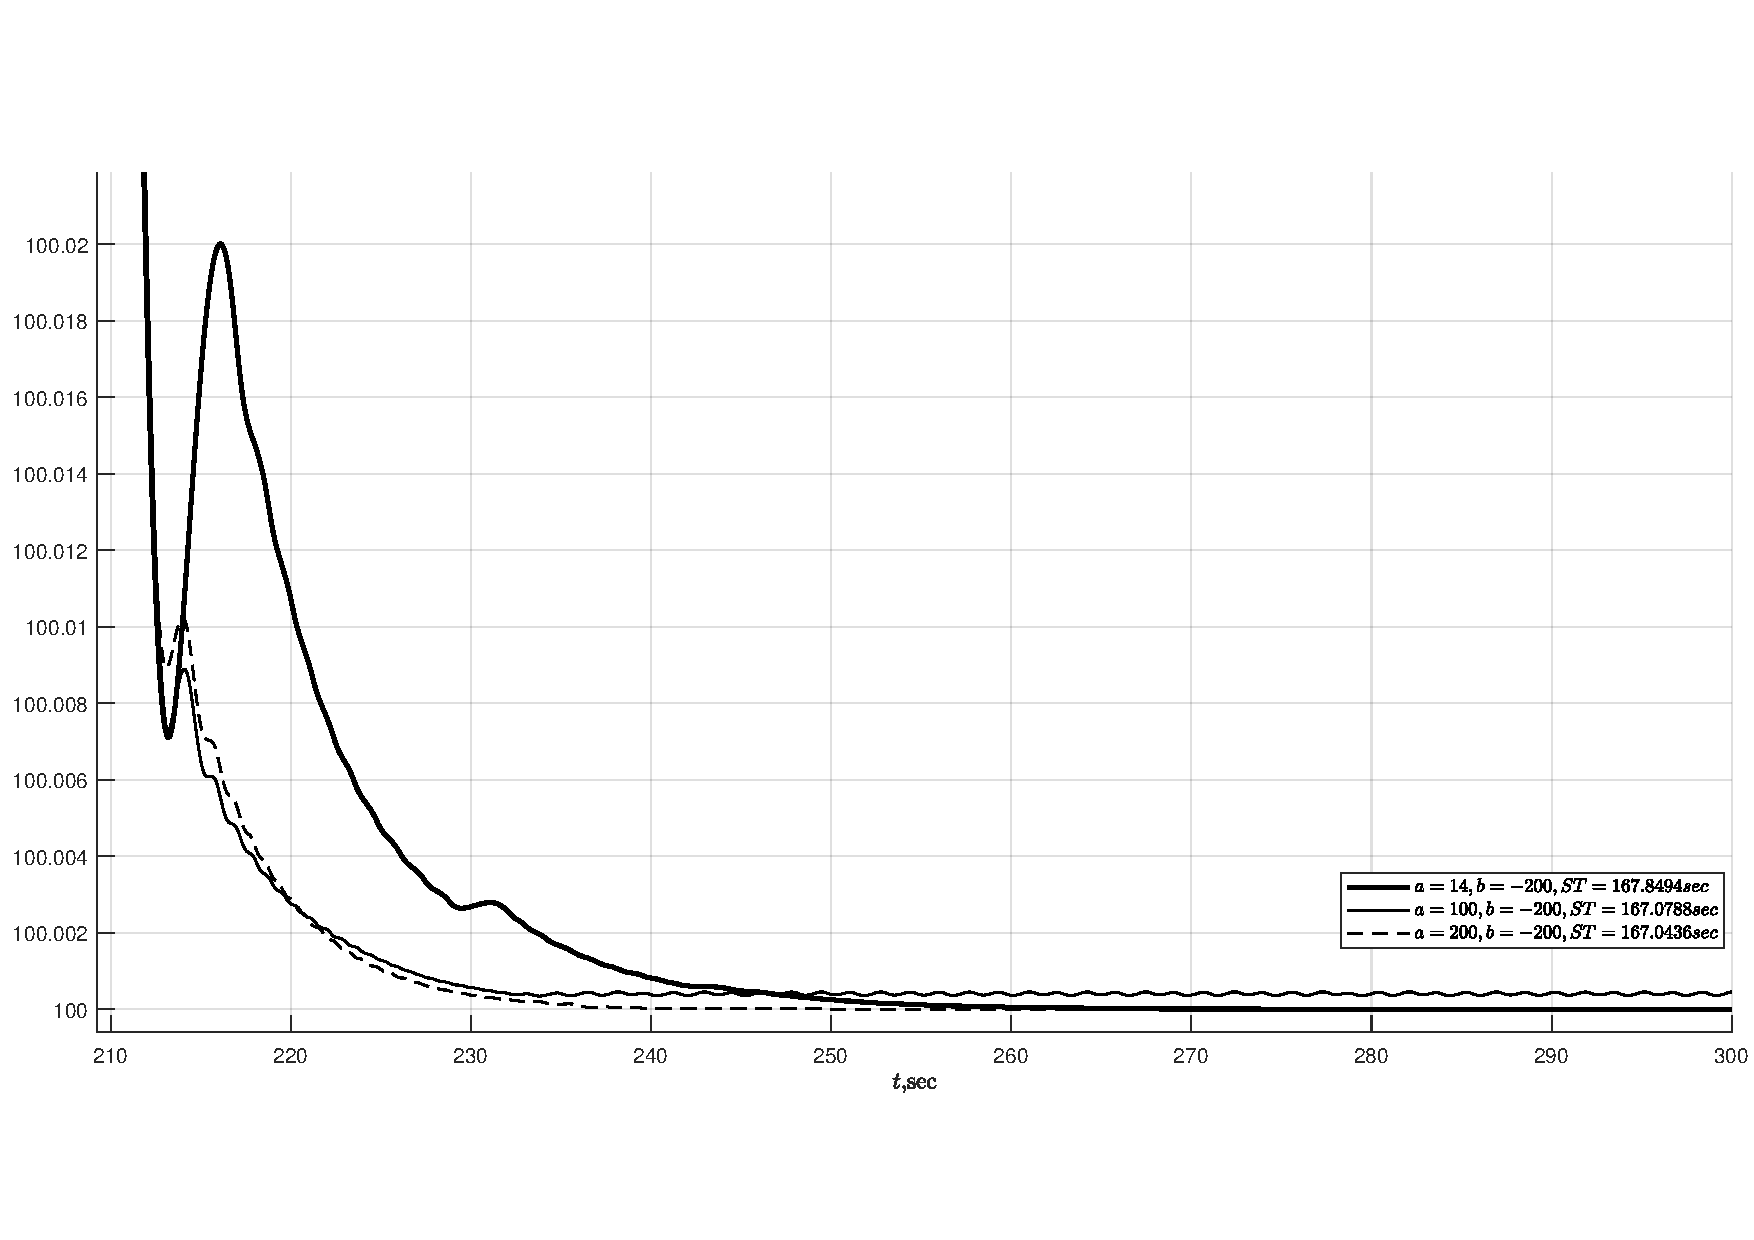
\includegraphics[width=1\linewidth]{images/final_VSS_PWM_a_zoom}
	\caption{ Увеличенные графики ПП при вариации параметров $a$ в <<малом>> в схеме с ШИМ.}\label{fig:final_VSS_PWM_a_zoom}
\end{figure}

Период квантования влияет на колебания системы в установвившемся состоянии, при его увеличении колебания уменьшаются.
Путем последовательных 
приближений было определено значение периода квантования $T{\text{кр}}$, при 
котором устойчивая без модулятора система становится неустойчивой, оно равно 4 сек.
На рис.\ref{fig:final_VSS_PWM_Ts45_gran} изображены переходный процессы при значениях, близких к $T{\text{кр}}$.

\begin{figure}[!h]\centering
	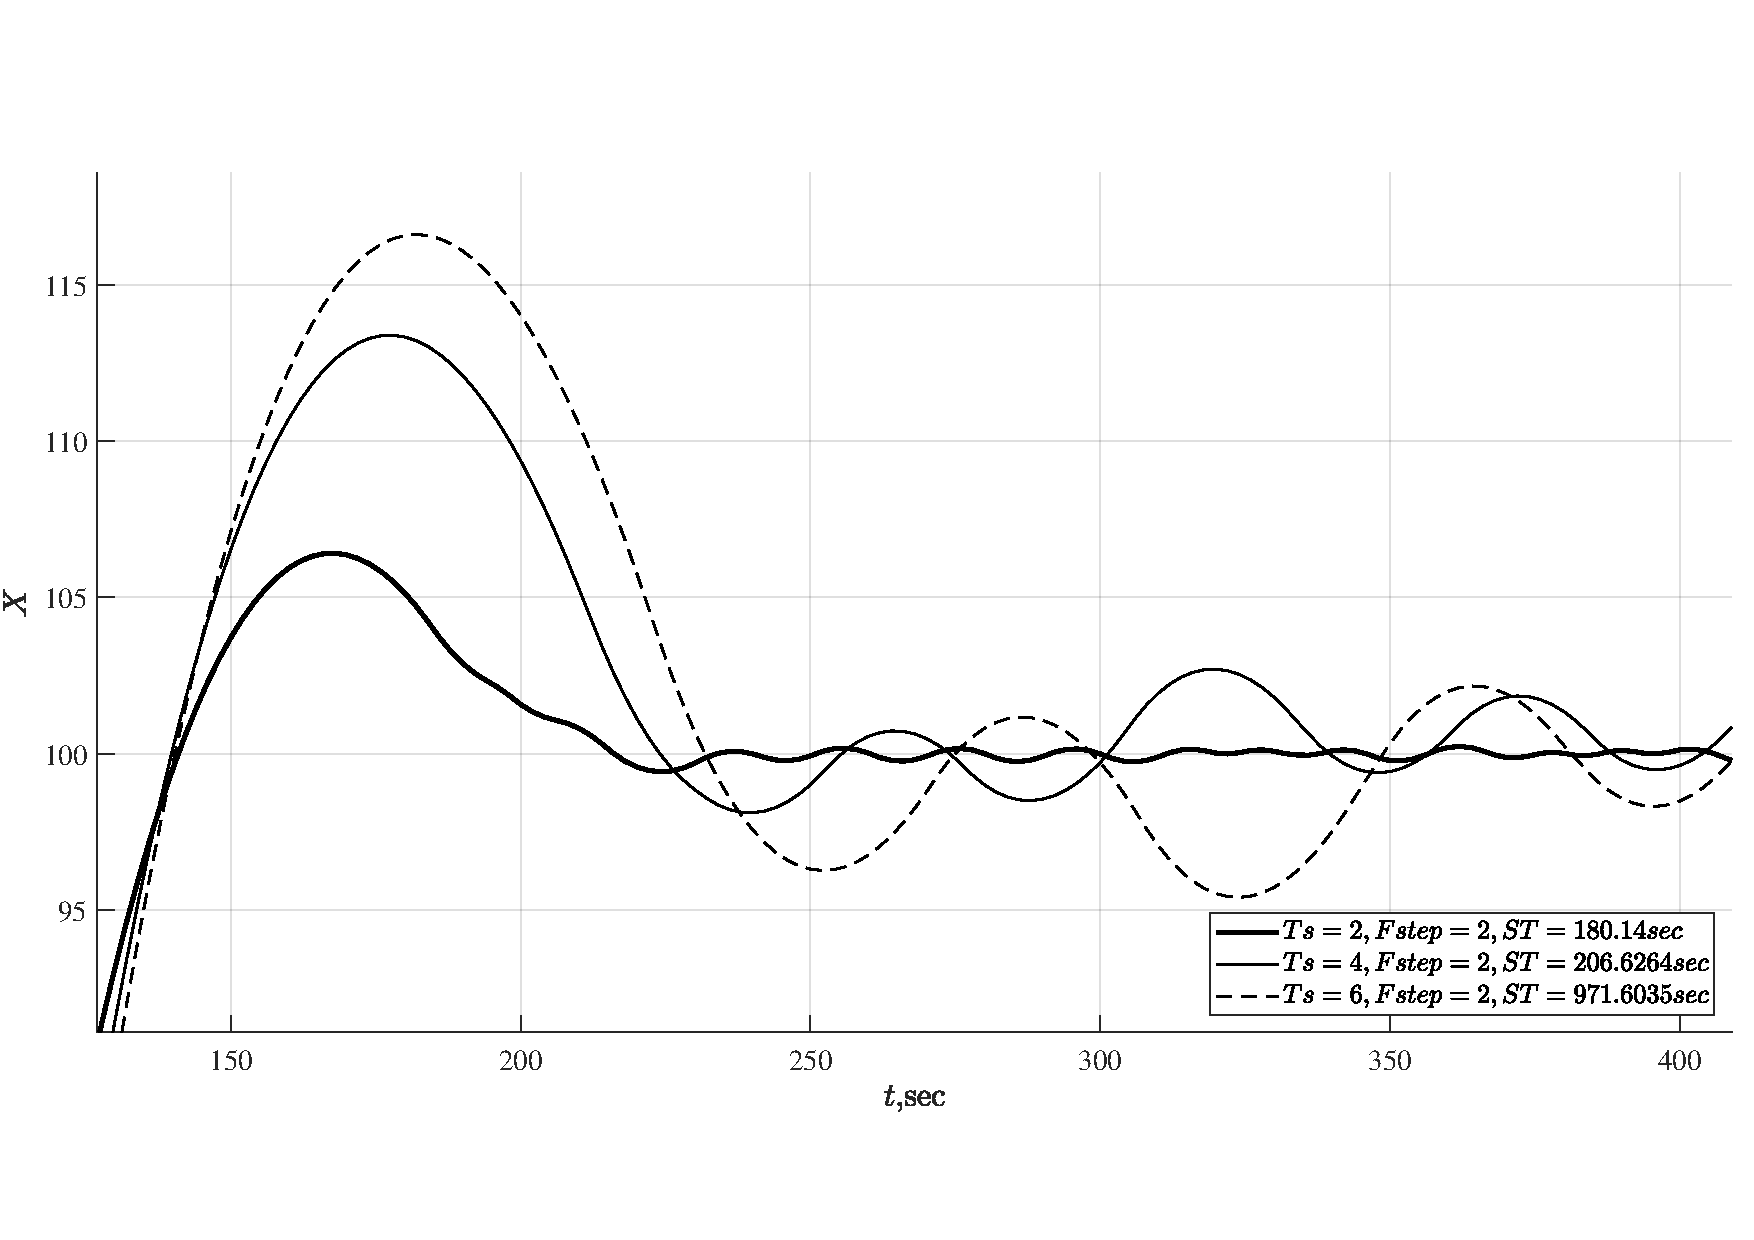
\includegraphics[width=1\linewidth]{images/final_VSS_PWM_Ts45_gran}
	\caption{ График переходного процесса при близких к $T_{\text{кр}}$ значениях.}\label{fig:final_VSS_PWM_Ts45_gran}
\end{figure}

Периода квантования $T_{\text{шим}}$, при котором система будет обладать теми же качествами, что и 
исходная равен 0,01 сек. Тогда соответствующий ему шаг решения равен 0,0001.  

Исследуем движение фазовых координат во времени посредством моделирования процессов в системе при отклонении системы от состояния равновесия. 
На рис.\ref{fig:final_VSS_PWM_sv_DCS_bol},\ref{fig:final_VSS_PWM_sv_DCS_mal} указано изменение выходной переменной. 
\begin{figure}[!h]\centering
	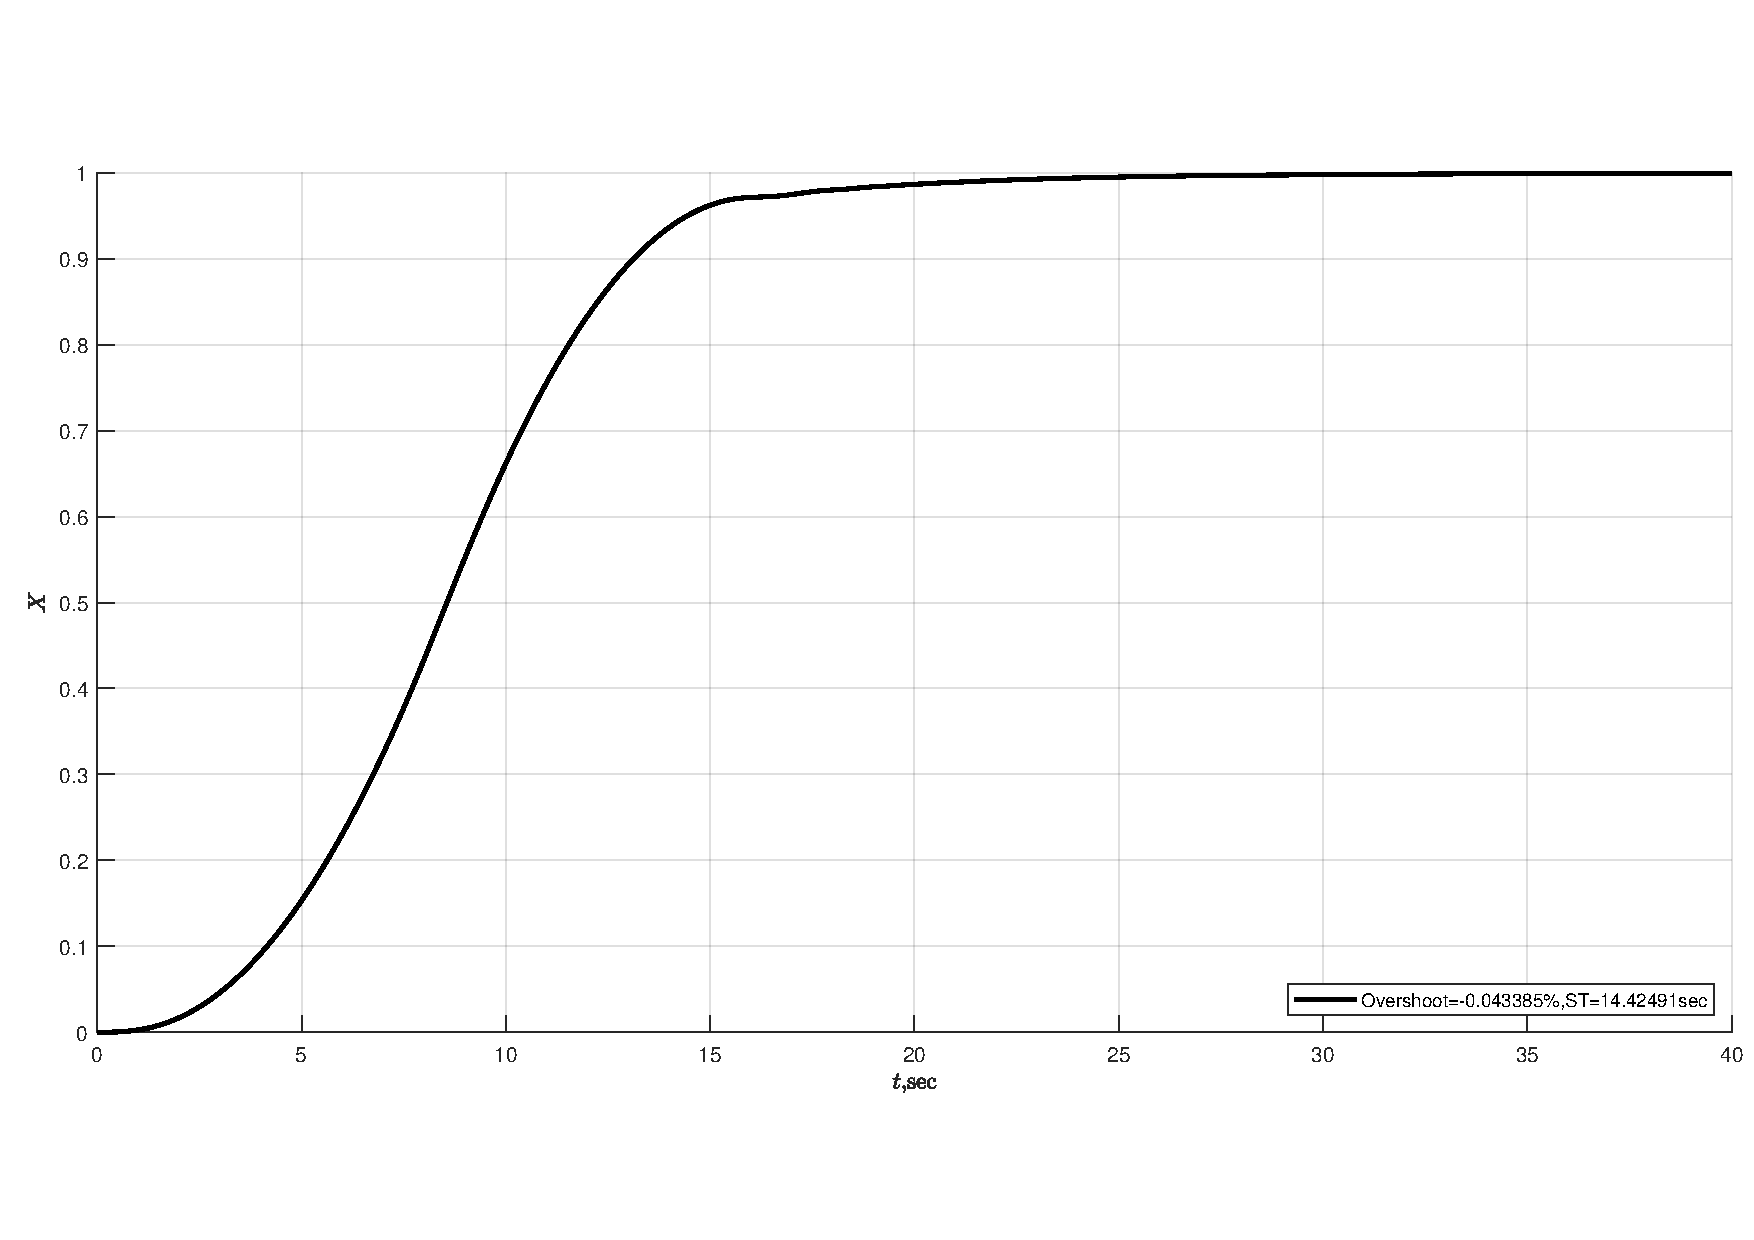
\includegraphics[width=1\linewidth]{images/final_VSS_PWM_sv_DCS_mal}
	\caption{ Графики изменения переменных состояния в <<малом>>.}\label{fig:final_VSS_PWM_sv_DCS_mal}
\end{figure}
\begin{figure}[!h]\centering
	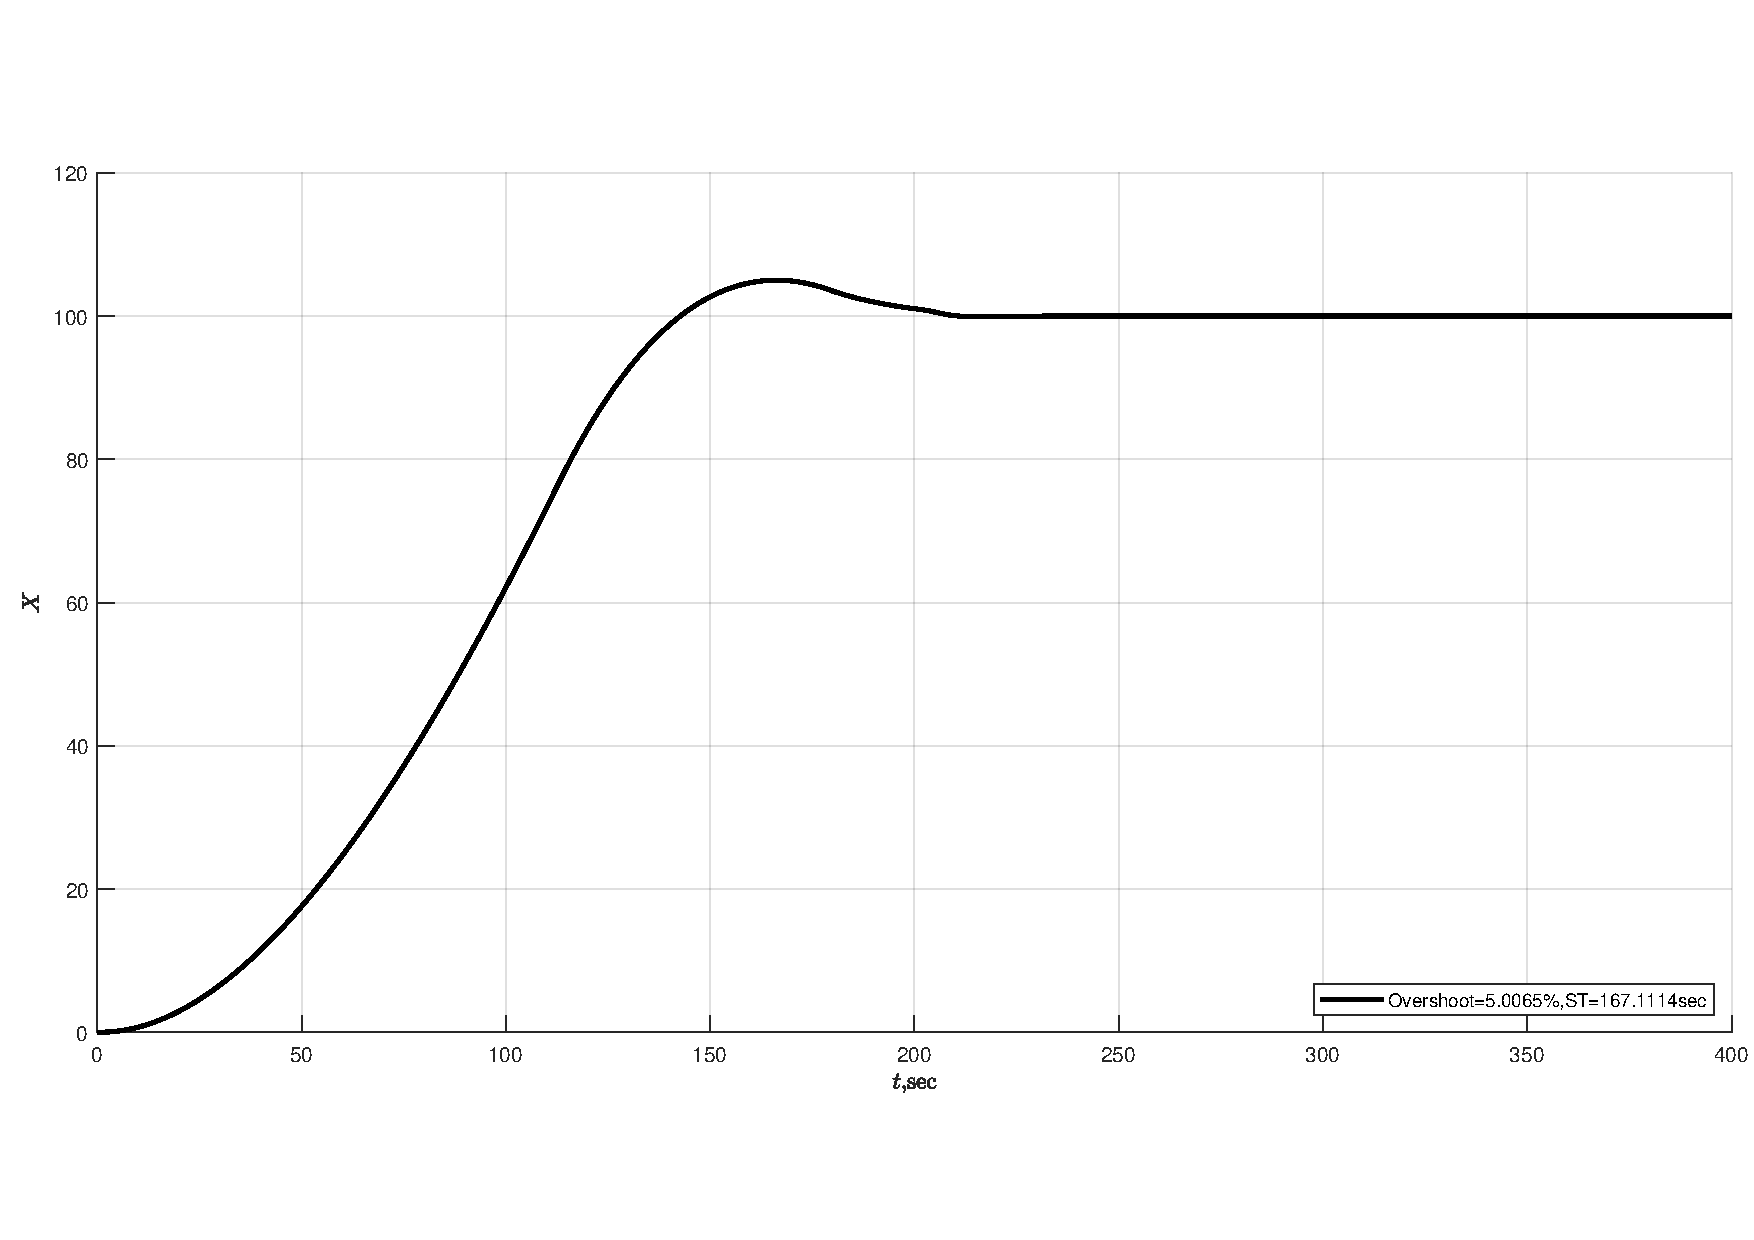
\includegraphics[width=1\linewidth]{images/final_VSS_PWM_sv_DCS_bol}
	\caption{ Графики изменения переменных состояния в <<большом>>.}\label{fig:final_VSS_PWM_sv_DCS_bol}
\end{figure}
\begin{figure}[!h]\centering
	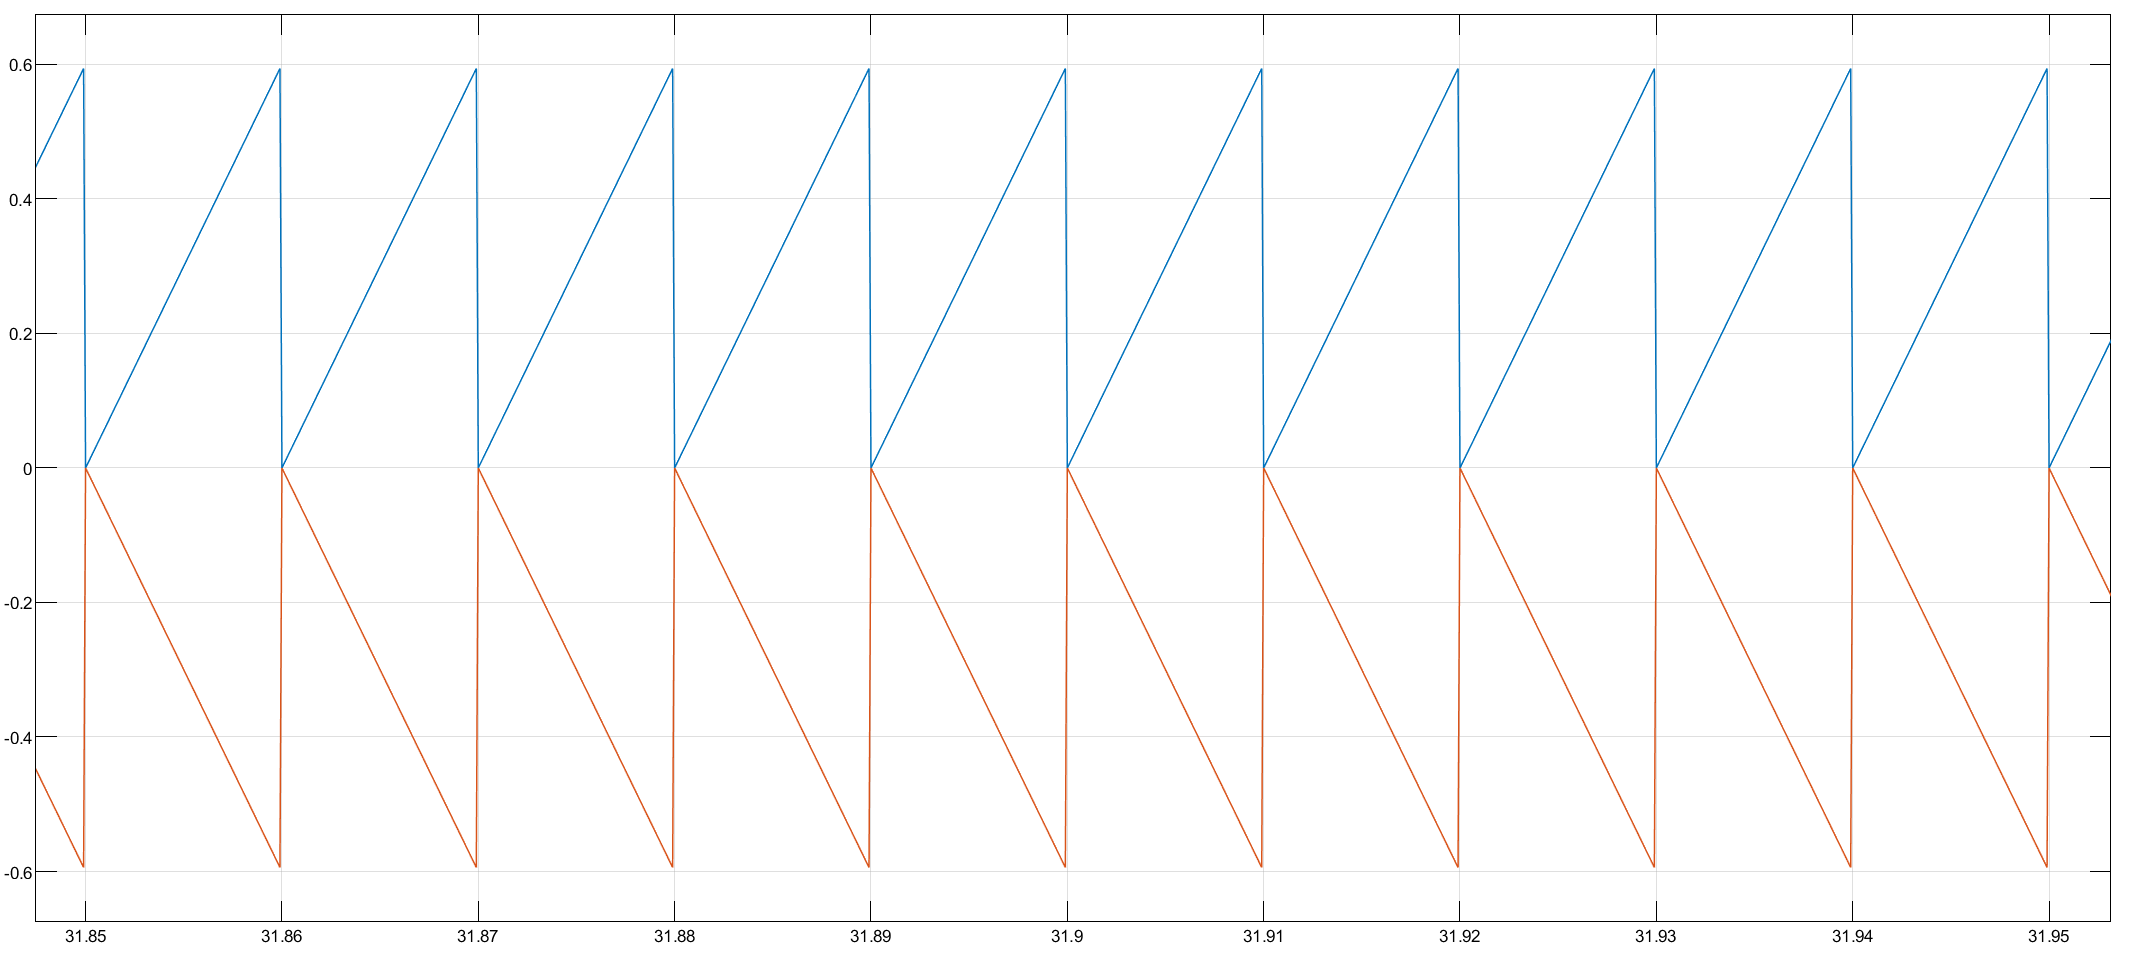
\includegraphics[width=0.6\linewidth]{images/final_VSS_PWM_DCS_SAW}
	\caption{ Генерируем пилу}\label{fig:final_VSS_PWM_DCS_SAW}
\end{figure}
Время переходного процесса при отклонении "в малом" согласно рисунку рис.\ref{fig:final_VSS_PWM_sv_DCS_mal} равно 14.42 сек.
Время переходного процесса при отклонении "в большом" согласно рисунку рис.\ref{fig:final_VSS_PWM_sv_DCS_bol} равно 167 сек.
В результате видим, что переходный процесс по прежнему удовлетворяет условиям задания.
\begin{figure}[!h]\centering
	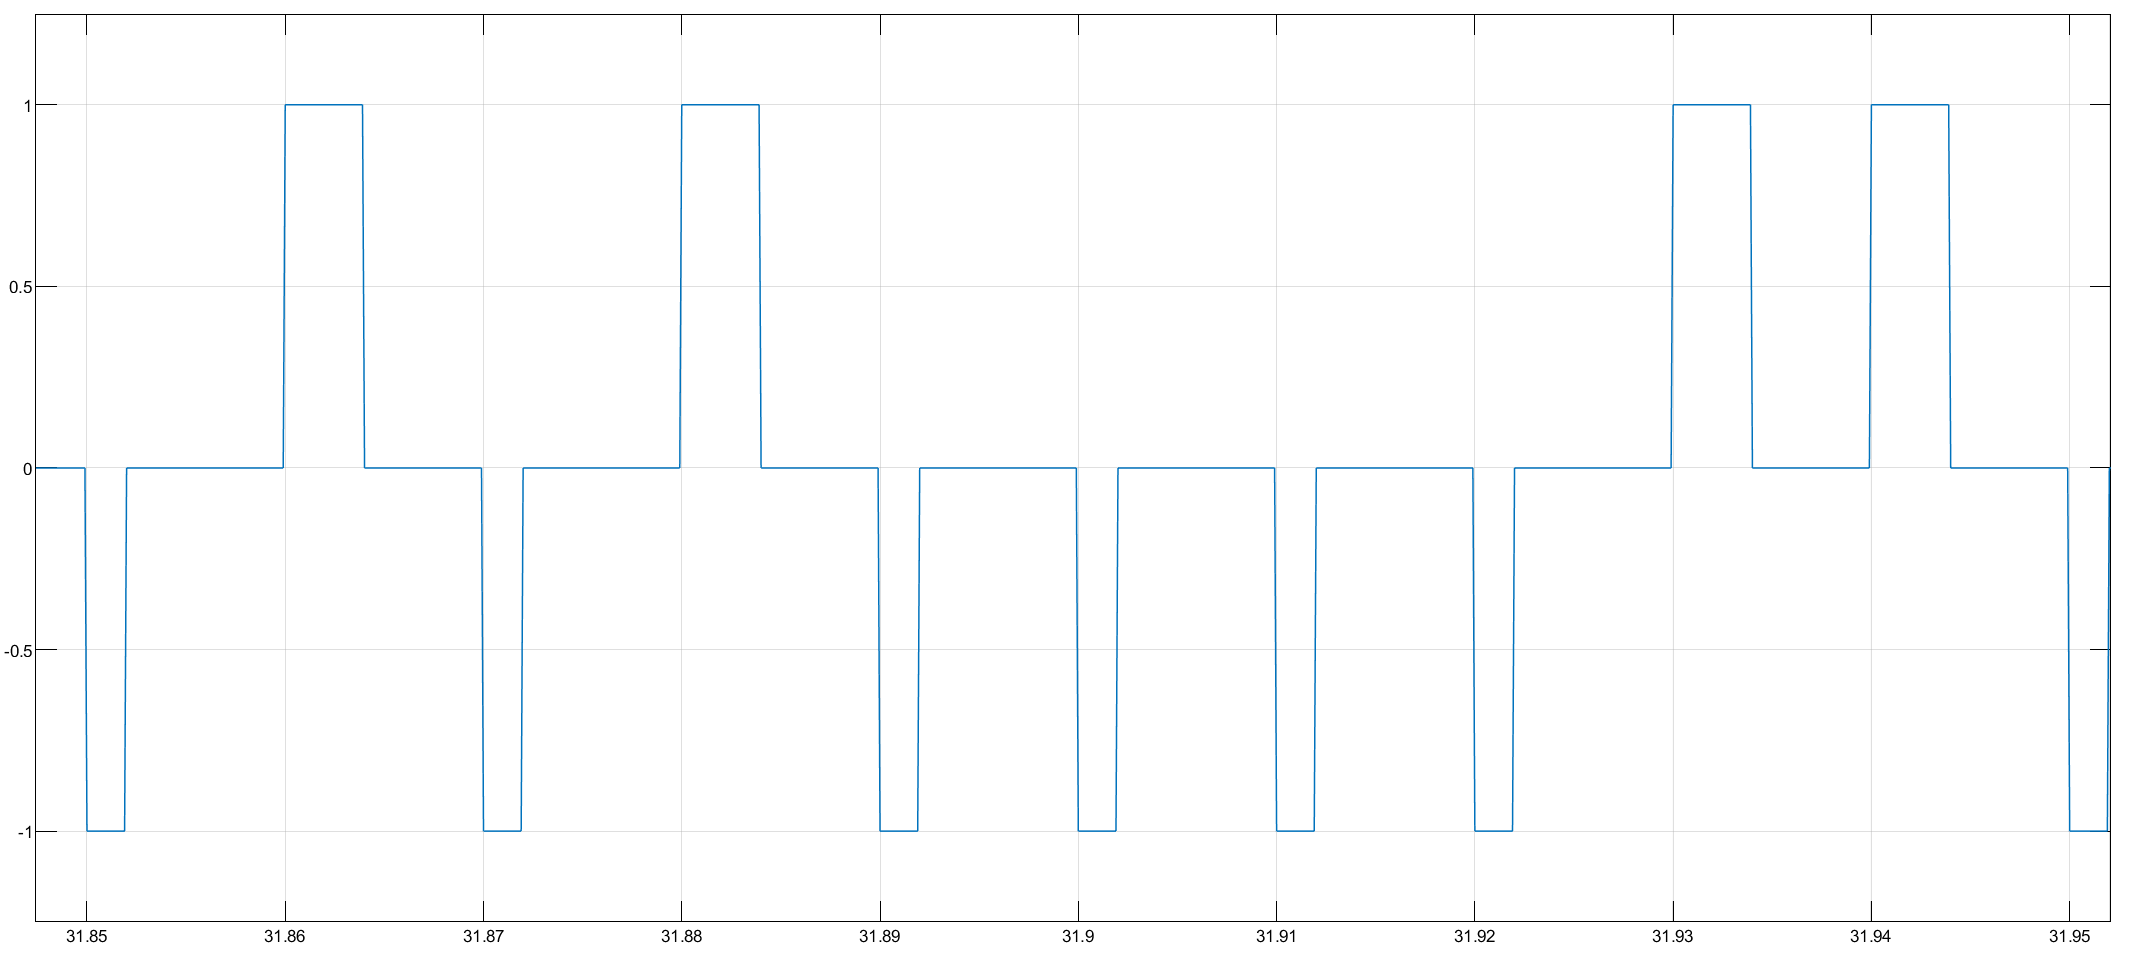
\includegraphics[width=0.6\linewidth]{images/final_VSS_PWM_DCS_PWM}
	\caption{ Воздействие на объект (ШИМ)}\label{fig:final_VSS_PWM_DCS_PWM}
\end{figure}
\begin{figure}[!h]\centering
	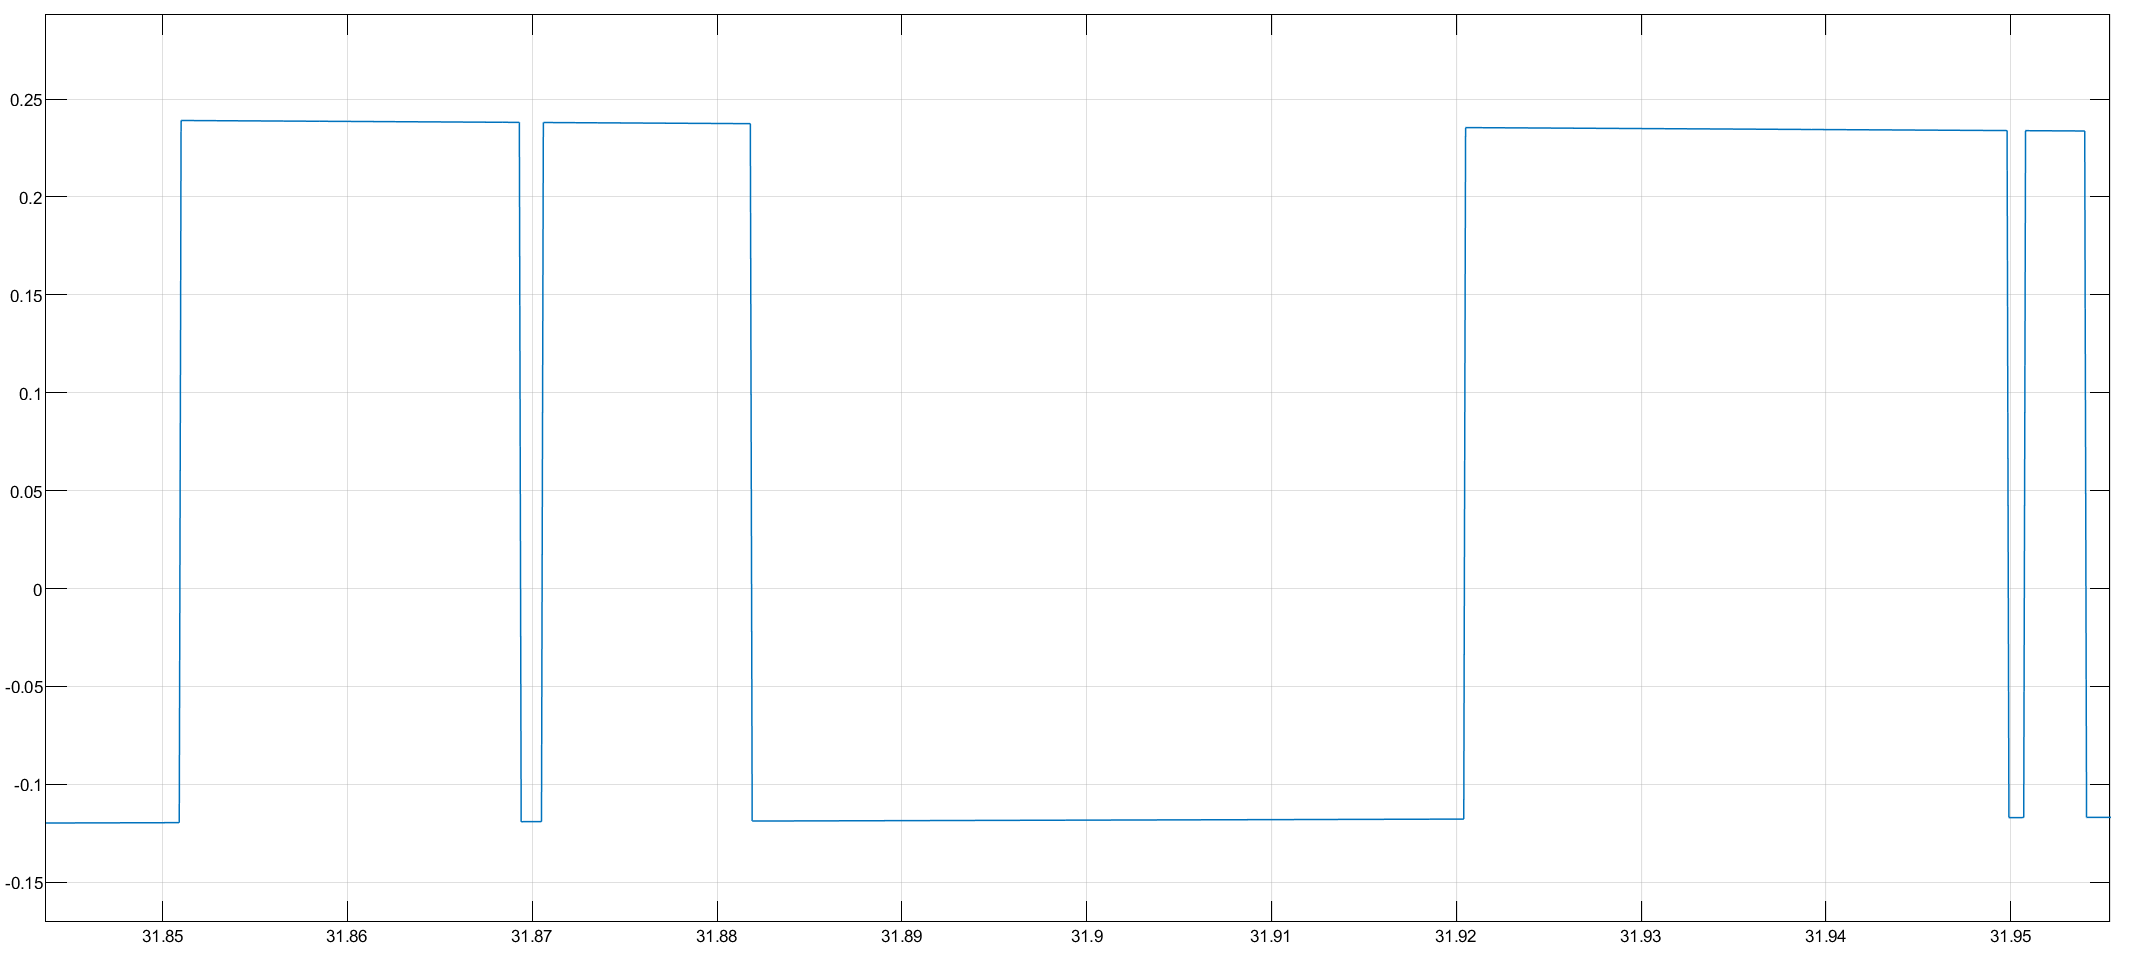
\includegraphics[width=0.6\linewidth]{images/final_VSS_PWM_DCS_upr}
	\caption{ управляющий непрерывный сигнал }\label{fig:final_VSS_PWM_DCS_upr}
\end{figure}
\begin{figure}[!h]\centering
	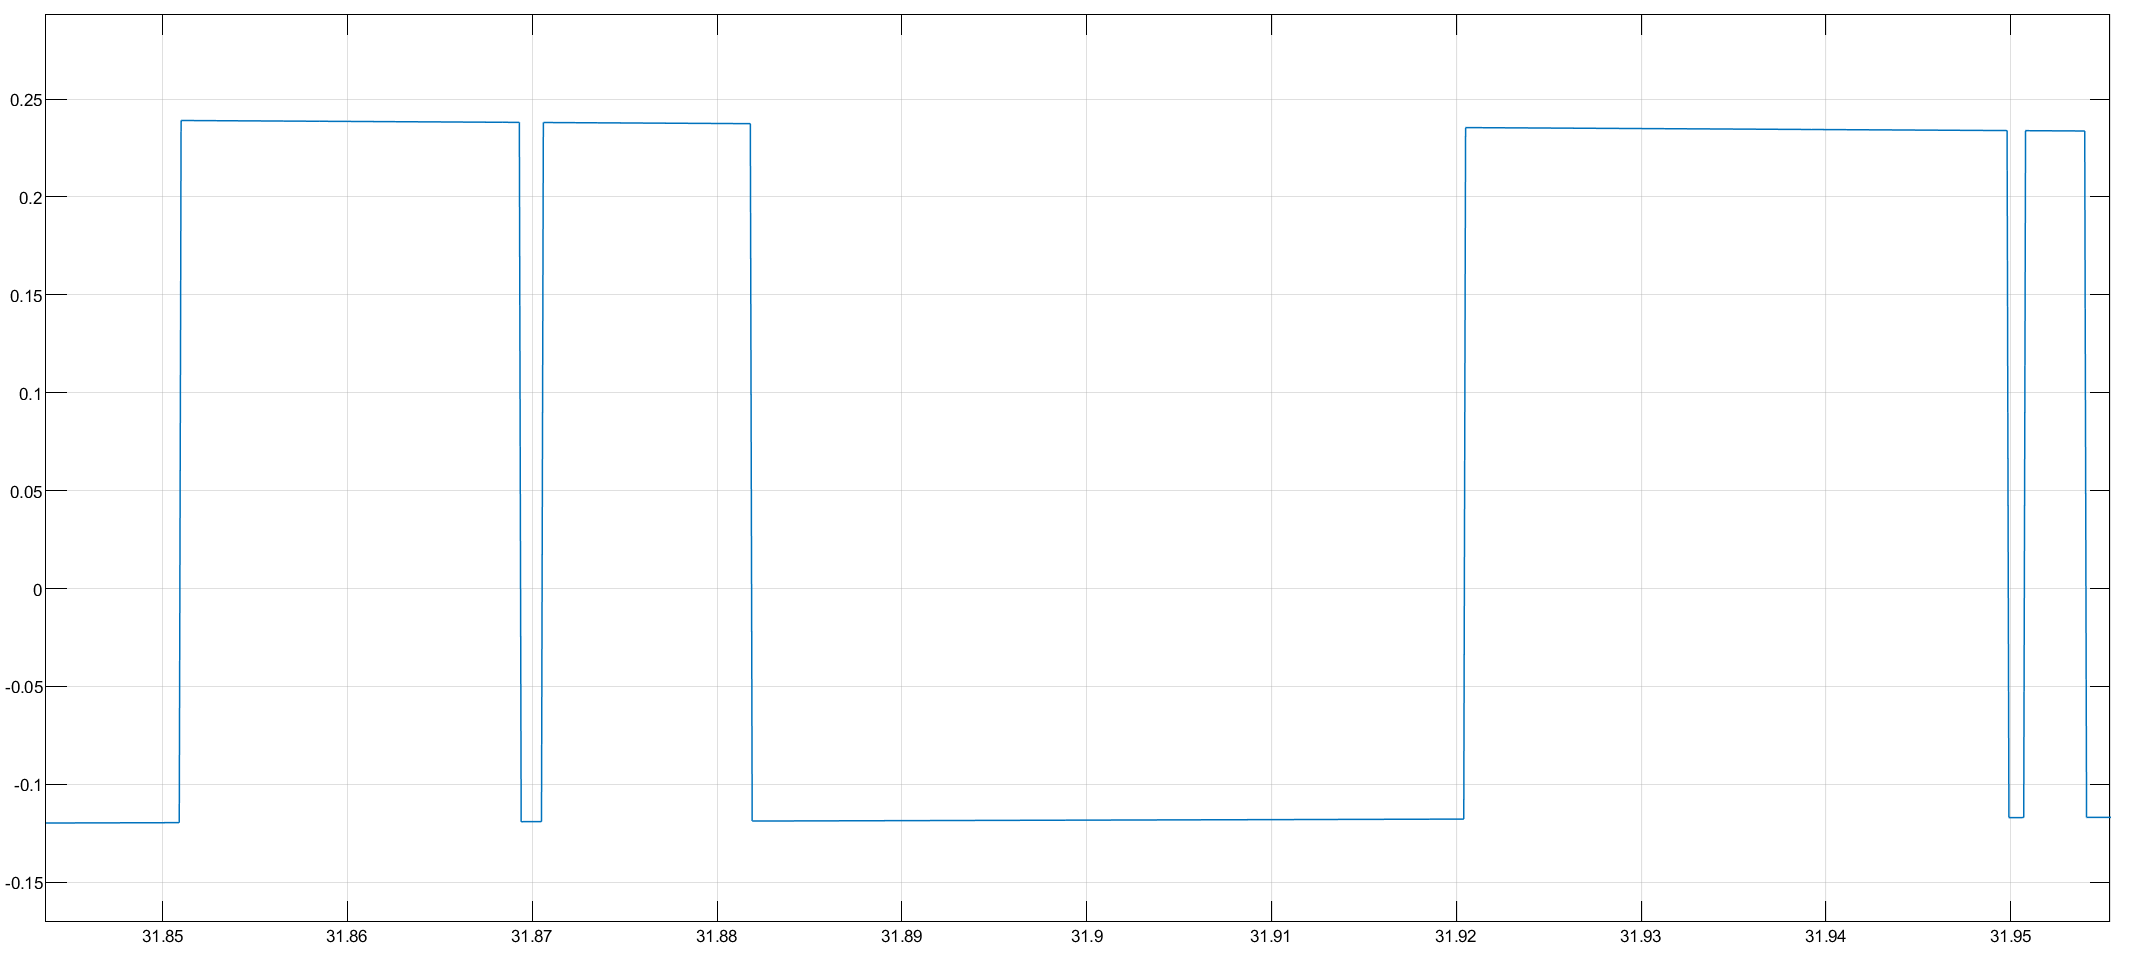
\includegraphics[width=0.6\linewidth]{images/final_VSS_PWM_DCS_upr_ogr}
	\caption{ управляющий непрерывный сигнал после насыщения}\label{fig:final_VSS_PWM_DCS_upr_ogr}
\end{figure}
\begin{figure}[!h]\centering
	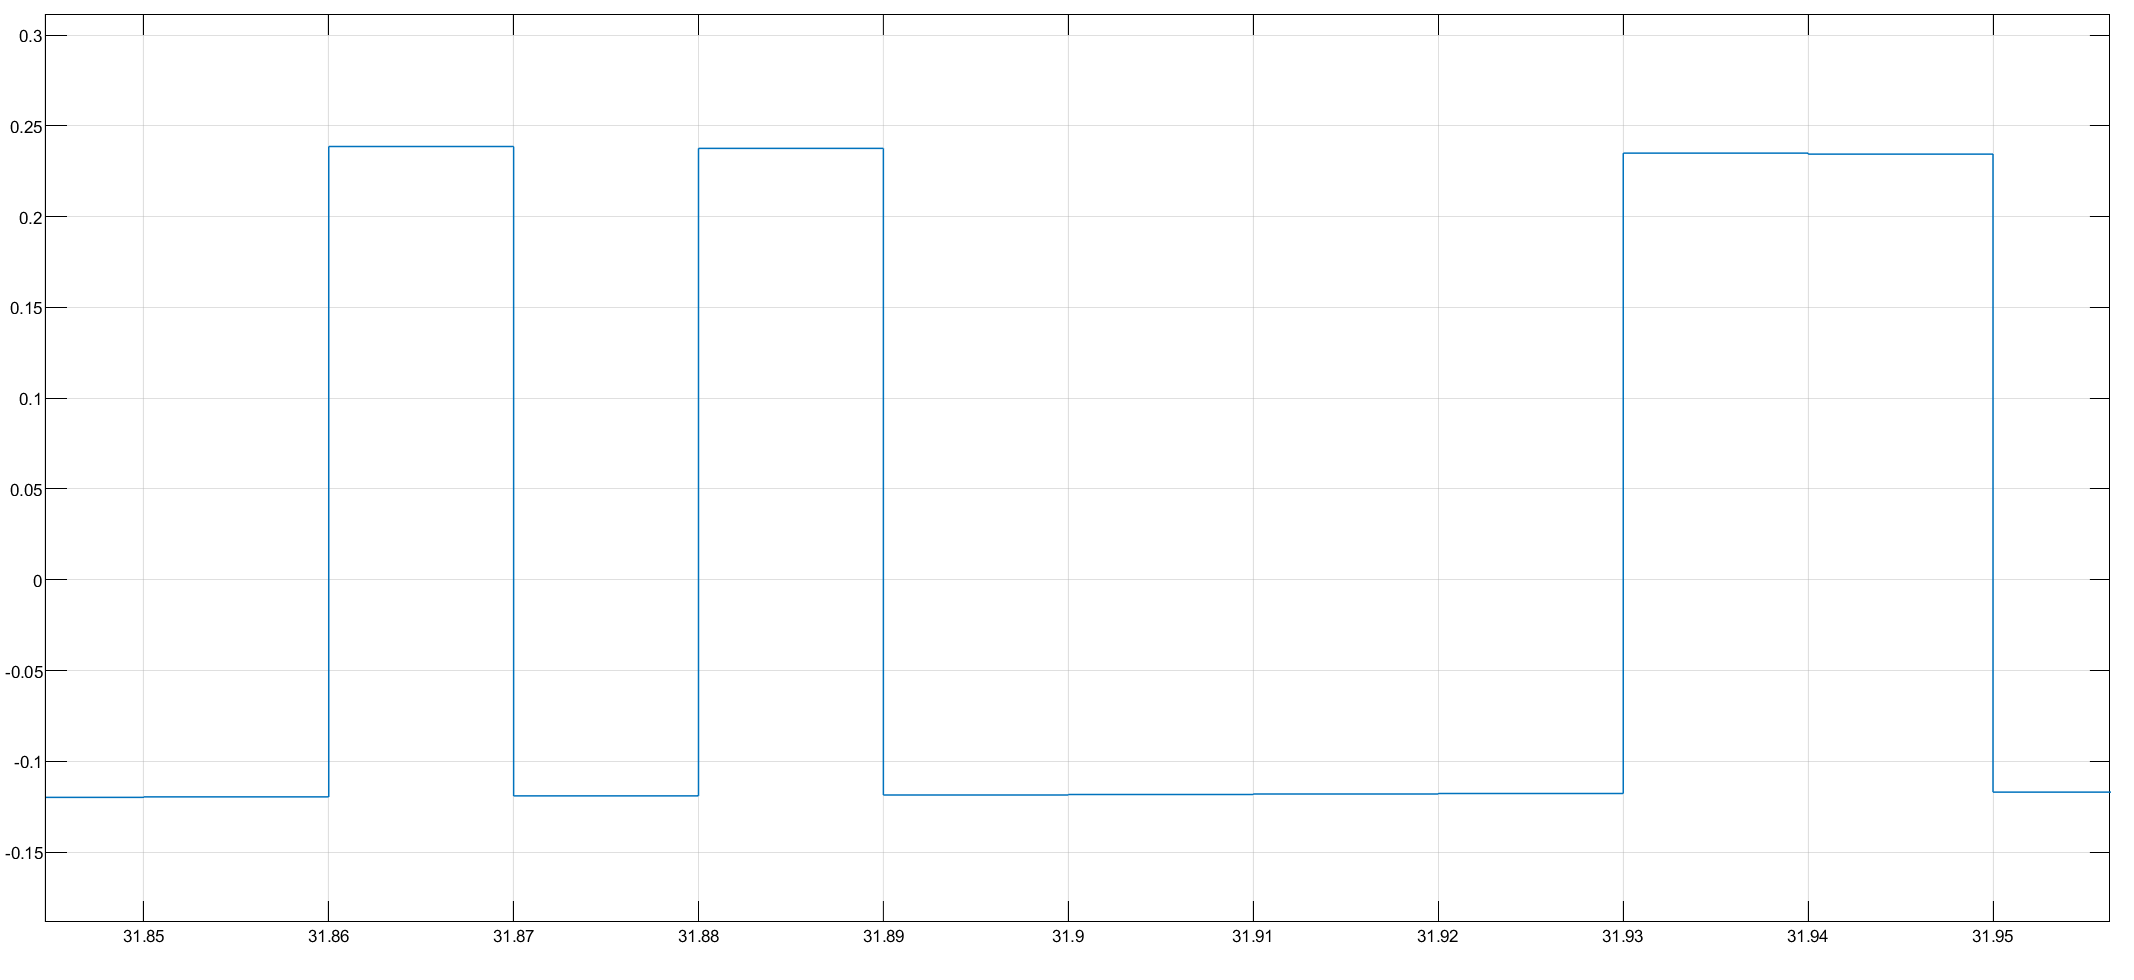
\includegraphics[width=0.6\linewidth]{images/final_VSS_PWM_DCS_upr_ogr_dig}
	\caption{ управляющий дискретизированный сигнал }\label{fig:final_VSS_PWM_DCS_upr_ogr_dig}
\end{figure}

